\documentclass[10pt,twocolumn]{article}
\usepackage{times}
\usepackage{array}
\newcolumntype{L}[1]{>{\raggedright\let\newline\\\arraybackslash\hspace{0pt}}m{#1}}
\usepackage{arydshln}
\usepackage{geometry}
\usepackage{balance}
\usepackage{enumitem}
% \usepackage{hyperref}

% Our inputs/packages
\usepackage[utf8]{inputenc}
\usepackage{multirow}
\usepackage{graphicx}
\usepackage{listings}
\usepackage{url}
\usepackage{amsmath}
\usepackage{color}
\usepackage{tabularx}
\usepackage{caption}
\usepackage{subcaption}
\usepackage{tikz}
\usetikzlibrary{arrows,decorations.pathmorphing,backgrounds,fit,positioning,shapes.symbols,chains,shapes.geometric,shapes.arrows,calc}


\newcommand{\ra}{$\rightarrow$}
\newboolean{showedits}
\setboolean{showedits}{true} % toggle to show or hide edits
\ifthenelse{\boolean{showedits}}
{
	\newcommand{\ugh}[1]{\textcolor{red}{\uwave{#1}}} % please rephrase
	\newcommand{\ins}[1]{\textcolor{blue}{\uline{#1}}} % please insert
	\newcommand{\del}[1]{\textcolor{red}{\sout{#1}}} % please delete
	\newcommand{\chg}[2]{\textcolor{red}{\sout{#1}}{\ra}\textcolor{blue}{\uline{#2}}} % please change
}{
	\newcommand{\ugh}[1]{#1} % please rephrase
	\newcommand{\ins}[1]{#1} % please insert
	\newcommand{\del}[1]{} % please delete
	\newcommand{\chg}[2]{#2}
}

\newboolean{showcomments}
%\setboolean{showcomments}{true}
\setboolean{showcomments}{true}
\newcommand{\id}[1]{$-$Id: scgPaper.tex 32478 2010-04-29 09:11:32Z oscar $-$}
\newcommand{\yellowbox}[1]{\fcolorbox{gray}{yellow}{\bfseries\sffamily\scriptsize#1}}
\newcommand{\triangles}[1]{{\sf\small$\blacktriangleright$\textit{#1}$\blacktriangleleft$}}
\ifthenelse{\boolean{showcomments}}
%{\newcommand{\nb}[2]{{\yellowbox{#1}\triangles{#2}}}
{\newcommand{\nbc}[3]{
 {\colorbox{#3}{\bfseries\sffamily\scriptsize\textcolor{white}{#1}}}
 {\textcolor{#3}{\sf\small$\blacktriangleright$\textit{#2}$\blacktriangleleft$}}}
 \newcommand{\version}{\emph{\scriptsize\id}}}
{\newcommand{\nbc}[3]{}
 \renewcommand{\ugh}[1]{#1} % please rephrase
 \renewcommand{\ins}[1]{#1} % please insert
 \renewcommand{\del}[1]{} % please delete
 \renewcommand{\chg}[2]{#2} % please change
 \newcommand{\version}{}}
\newcommand{\nb}[2]{\nbc{#1}{#2}{orange}}

\definecolor{ibcolor}{rgb}{0.9,0.5,0}
\definecolor{jscolor}{rgb}{1,0,1}

%% \definecolor{bocolor}{rgb}{0.6,0.9,0.2}
%% \definecolor{jrcolor}{rgb}{0.5,0,0.5}
%% \definecolor{hkcolor}{rgb}{0.4,0.1,0}
%% \definecolor{nrcolor}{rgb}{1.0,0.6,0.1}
\definecolor{tdcolor}{rgb}{1.0,0,0}

\newcommand\ivan[1]{\nbc{IB}{#1}{ibcolor}}
\newcommand\jodi[1]{\nbc{JS}{#1}{jscolor}}
\newcommand\todo[1]{\nbc{TODO}{#1}{tdcolor}}

%%\newcommand{\ars}[1]{\textcolor{magenta}{[[#1]]}} 
%% \newcommand\dm[1]{\nbc{DM}{#1}{dmcolor}}
%% \newcommand\tg[1]{\nbc{TG}{#1}{tgcolor}}
%% \newcommand\kb[1]{\nbc{KB}{#1}{kbcolor}}

%\usepackage{wasysym}[nointegrals]

\newcommand\yesml[1]{\nbc{ML {\textcolor{yellow}\sun}}{#1}{mircolor}}

% End our inputs/packages

% do not change these values
\baselineskip 12pt
\textheight 9in
\textwidth 6.5in
\oddsidemargin 0in
\topmargin 0in
\headheight 0in
\headsep 0in
% end of do not change these values

% Custom commands
% NOTE: when using the bifrost command and you want a space after the word
% (i.e., Bifrost in), you must use {\bifrost} or it won't put a space
\newcommand{\dinv}{Dinv}
\newcolumntype{Y}{>{\raggedright\arraybackslash}X}


\definecolor{lightgray}{rgb}{.9,.9,.9}
\definecolor{darkgray}{rgb}{.4,.4,.4}
\definecolor{purple}{rgb}{0.65, 0.12, 0.82}
\definecolor{mygray}{rgb}{0.5,0.5,0.5}
\definecolor{mygreen}{rgb}{0,0.6,0}

\lstdefinelanguage{P4}{
   keywords={header_type,valid,control,action,modify_field,if,then,else,else if,or,and,not,while,do,apply,table},
   keywordstyle=\color{blue}\bfseries,
   identifierstyle=\color{black},
   sensitive=false,
   commentstyle=\color{mygreen}\ttfamily,
   comment=[l]{--},%
}

\lstset{
  language=P4,
  extendedchars=true,
  basicstyle=\scriptsize\ttfamily,
  showstringspaces=false,
  showspaces=false,
  numbers=left,
  numberstyle=\tiny\color{darkgray},
  numbersep=2pt,
  tabsize=1,
  breaklines=true,
  showtabs=false,
  captionpos=b,
  numberblanklines=false,
  escapeinside=\[\]
}

\def\outline{0} % 0 = full paper, 1 = outline
\def\thesis{0} % 0 = socc paper, 1 = thesis

\begin{document}

\title{Title}
\author{
        author 1,
        author 2
        \\
\small {\em  
		Dept. of Computer Science, University of British Columbia 
        } \\ [2mm]
\small Submission Type: Research
}
\date{}
\maketitle


\if\outline1
	\input{outline.tex}
\else
	\chapter{Abstract}
\label{sec:abstract}

Internet censorship is a form of digital authoritarianism in certain countries that restrict access to the internet. Internet freedom, to a degree, is possible even in these countries by means of proxies maintained outside of the censor's boundaries. These proxies can be compromised by censors who pose as legitimate users to discover proxies. Censors are powerful adversaries and may block access to any proxy once they know about it.

We propose a novel technique to address the proxy distribution problem in this thesis. We introduce the \textit{needle} algorithm that preserves proxies by limiting their distribution. The number of proxies preserved is controlled by the algorithm's parameters. We show that it is a useful mechanism for preserving proxies under a censorship threat model. 

We examine characteristics of the algorithm in a simulation. Three measures are important under the censorship threat model; the enumeration or discovery of all proxies, load balancing, and the collateral damage of innocent bystanders. We compare the results of these experiments with two well-known algorithms, uniform random and power of 2 choices, as well as Tor's \texttt{bridgedb} proxy assignment mechanism. 

    \input{acks.tex}
	\chapter{Introduction}
\label{sec:intro} 

%%%%%%%%%%%%%%%%%%%%%%%%%%%%%%%%%%%%%%%%%%%%%%%%%%%%%%%%%%%%%%%%%%%%%%
\begin{figure*}[h!]
\centering
     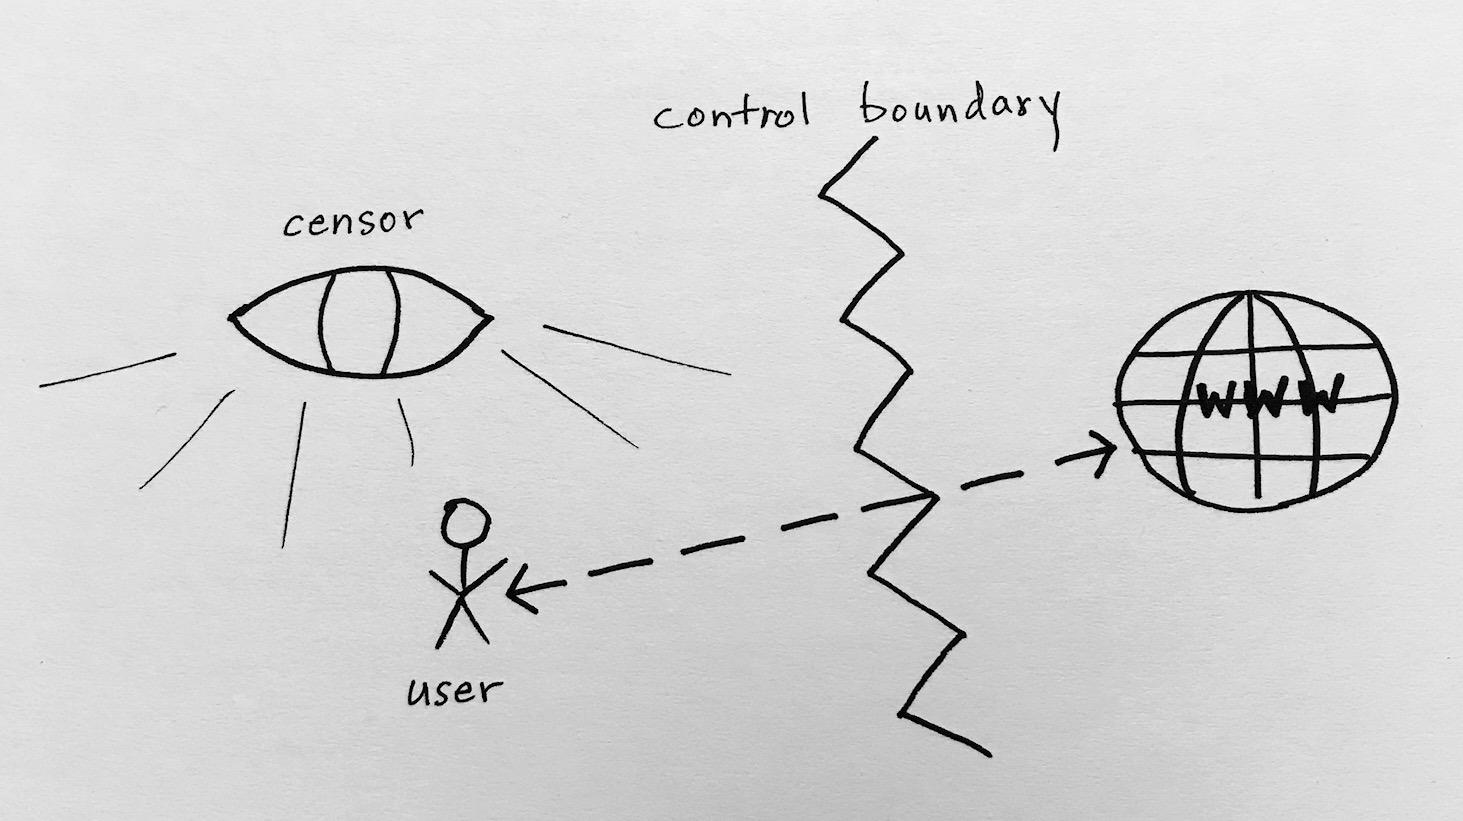
\includegraphics[width=1.0\textwidth]{fig/censor_simple.png}
    \caption{A censor observes a citizen's network activity to the internet outside its control boundary.}
    
    \label{fig:simplecensor}
\end{figure*}
%%%%%%%%%%%%%%%%%%%%%%%%%%%%%%%%%%%%%%%%%%%%%%%%%%%%%%%%%%%%%%%%%%%%%%

Internet censorship is a significant and growing problem that threatens our freedom of expression and access to information. A citizen within a censored country attempts to access the internet that is hosted beyond the censor's control boundary, shown in Figure \ref{fig:simplecensor}. A censor is a strong nation state adversary that conducts mass surveillance and utilizes blacklists. One of the simplest techniques employed by censors is to deny access to users by blocking traffic destined for blacklisted sites. 

%%%%%%%%%%%%%%%%%%%%%%%%%%%%%%%%%%%%%%%%%%%%%%%%%%%%%%%%%%%%%%%%%%%%%%
\begin{figure*}[h!]
\centering
     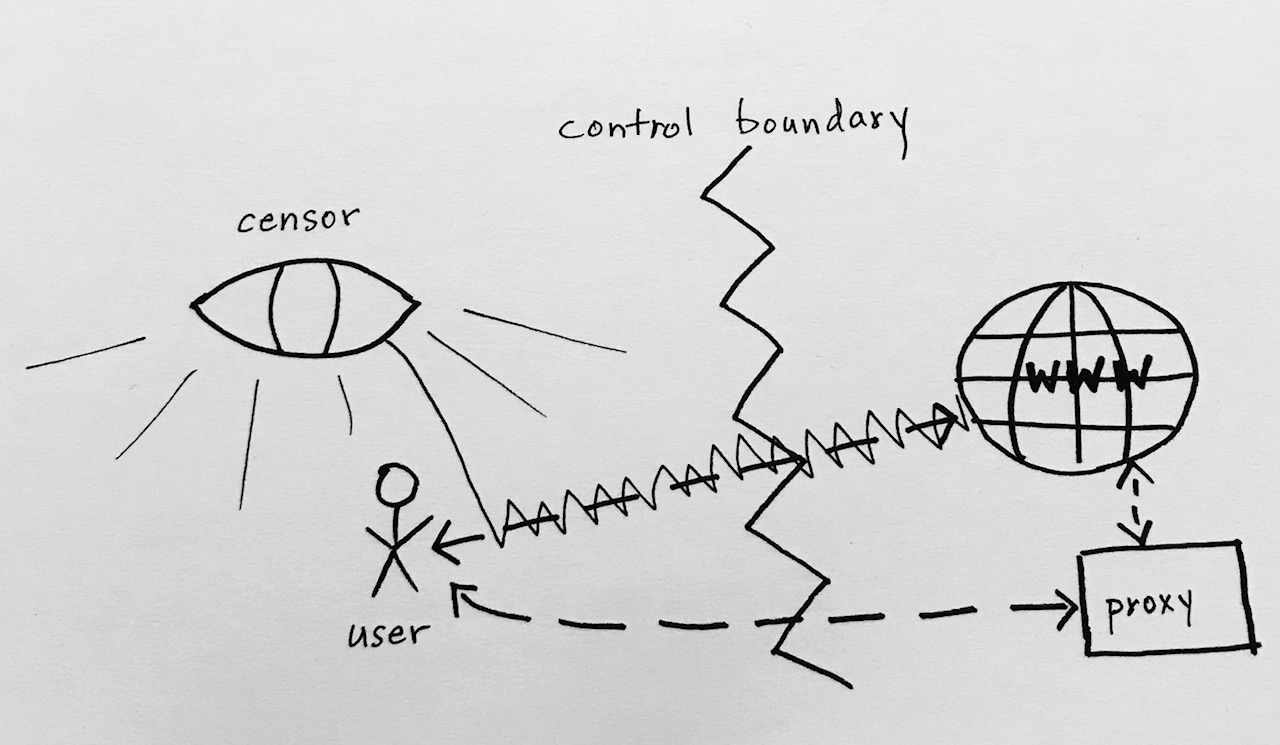
\includegraphics[width=1.0\textwidth]{fig/censor_block.png}
    \caption{A censor blocks direct access to a site but the citizen uses a proxy to access the internet.}
    
    \label{fig:censorblock}
\end{figure*}
%%%%%%%%%%%%%%%%%%%%%%%%%%%%%%%%%%%%%%%%%%%%%%%%%%%%%%%%%%%%%%%%%%%%%%

This effective censorship technique is circumvented by means of proxies; single-hop servers outside of the censored country that facilitate indirect access to censored information. In Figure \ref{fig:censorblock}, a citizen is blocked from the internet but manages to access sites via a proxy. Censorship resistance systems manage proxies and allow users in censored countries to access blacklisted websites. These systems bypass censors and route users through secret paths. Secret paths rely on proxies that are managed by censorship resistance systems. Proxies serve as intermediary hops between a user and a blacklisted destination site.

%%%%%%%%%%%%%%%%%%%%%%%%%%%%%%%%%%%%%%%%%%%%%%%%%%%%%%%%%%%%%%%%%%%%%%
\begin{figure*}[h!]
\centering
     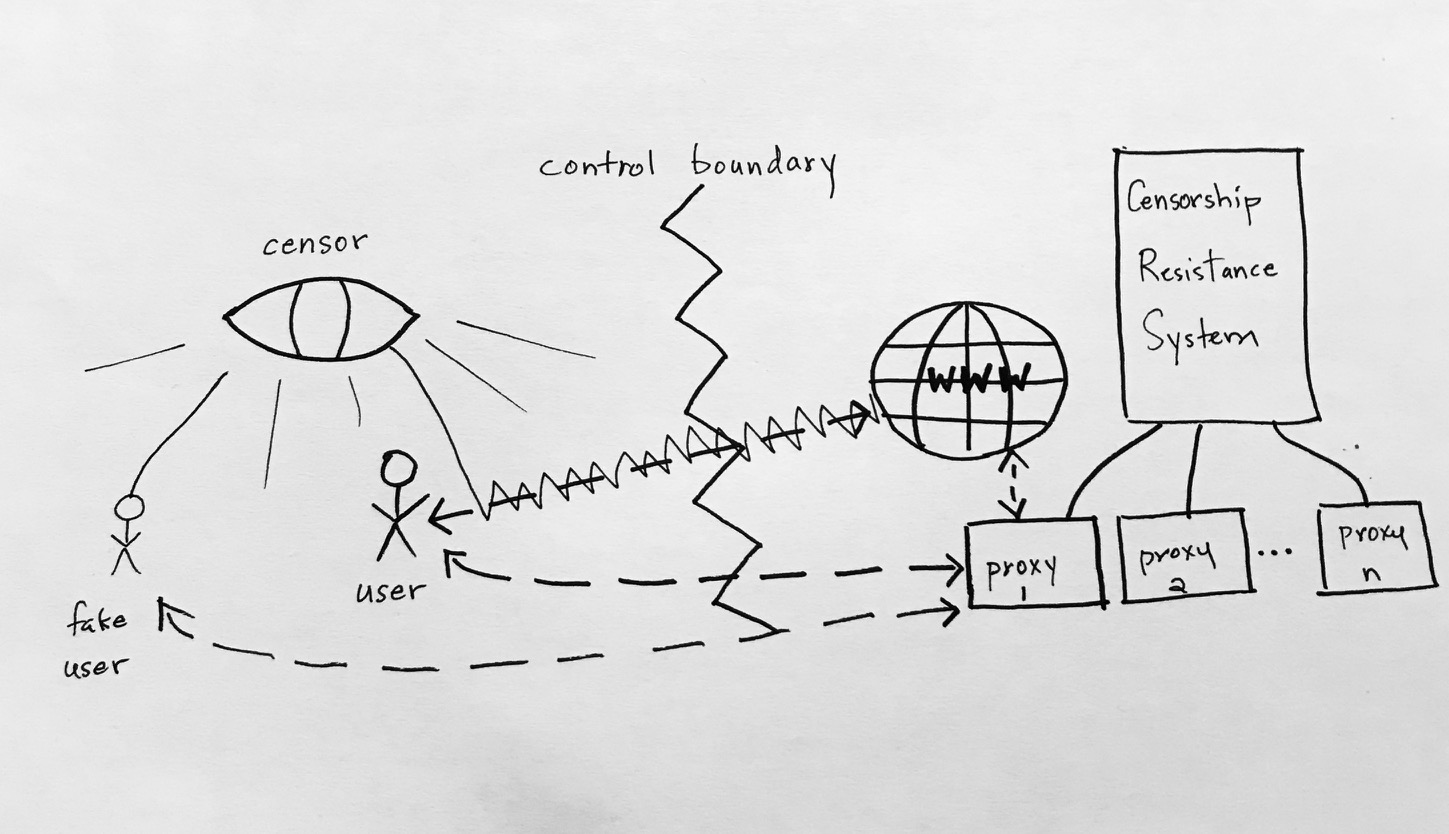
\includegraphics[width=1.0\textwidth]{fig/censor_crs.png}
    \caption{Censorship circumvention via proxy distribution.}
    \label{fig:proxydistro}
\end{figure*}
%%%%%%%%%%%%%%%%%%%%%%%%%%%%%%%%%%%%%%%%%%%%%%%%%%%%%%%%%%%%%%%%%%%%%

Censorship resistance systems are composed of honest and dishonest (fake) users, several honest proxies, and a centralized proxy distributor that is also honest. Figure \ref{fig:proxydistro} shows a typical censorship circumvention system using a collection of proxies and a centralized distributor. Censorship resistance systems rely on the proxy distributor to assign clients to proxies. Honest users anonymously request proxies and receive proxy information details from the distributor. However, a censor may also learn proxy details by posing as an honest user via legitimate, anonymous methods. The censor coordinates information collected through a collection of fake accounts to gain knowledge of the proxies in the circumvention system.

To get an idea of the scale of censorship events around the world, Figure \ref{fig:oonimap} shows a world map where the OONI project's network measurement tests, ooniprobes, are run daily by volunteers.\footnote{https://blog.torproject.org/tor-heart-ooni-project} The red areas on the map outline confirmed cases of censorship. Censorship is confirmed by the response body of an HTTP request of a blocked page from within a censored country.

%%%%%%%%%%%%%%%%%%%%%%%%%%%%%%%%%%%%%%%%%%%%%%%%%%%%%%%%%%%%%%%%%%%%%%
\begin{figure*}[h!]
\centering
     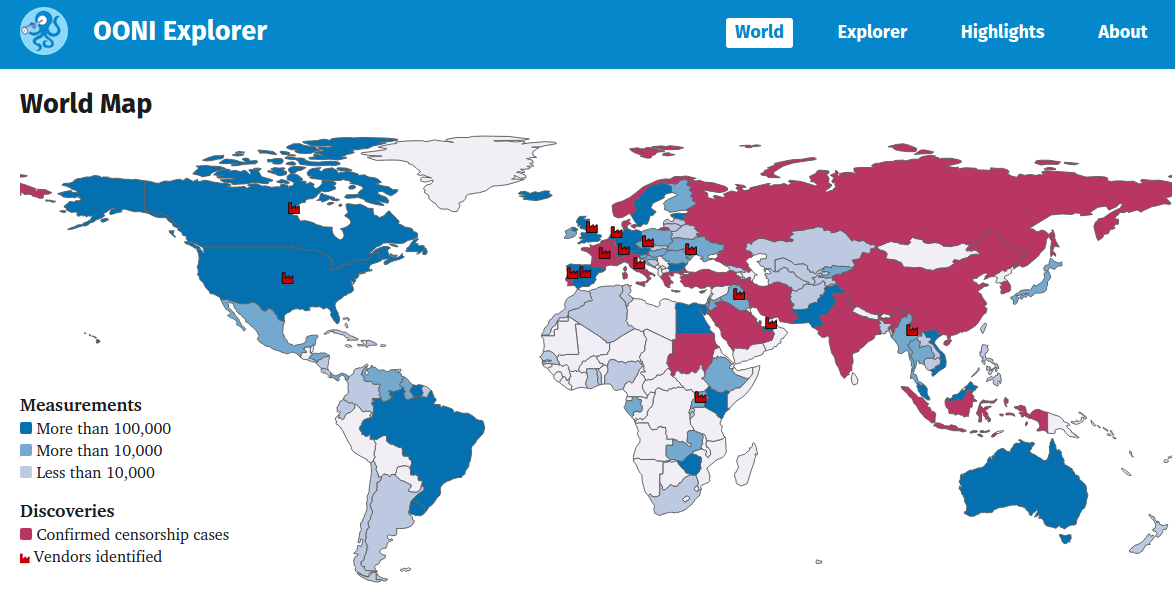
\includegraphics[width=1.0\textwidth]{fig/ooni_map.png}
    \caption{Tor's OONI project collects censorship event data.}
    
    \label{fig:oonimap}
\end{figure*}
%%%%%%%%%%%%%%%%%%%%%%%%%%%%%%%%%%%%%%%%%%%%%%%%%%%%%%%%%%%%%%%%%%%%%%

In our proxy distribution problem, we accept that proxies will be distributed to censors. Our goal is to provide service to clients while preserving some proxies from distribution. In this thesis, we introduce a lightweight approach for the proxy distribution problem to distribute proxies to clients while fake clients are present. We implement a scheme with the goal to maximize the resource loss of an attacker. Our approach uses principles of load balancing in a non-intuitive way to preserve random proxies by unbalancing the load on proxies, making them more difficult to discover. This approach operates on the pessimistic assumption that all proxies are destined for discovery over time in a system, where the system cannot distinguish between honest users and fake users. 
We provide an approximation of the censor's required effort to discover all of the proxies in a system based on the coupon collector problem\cite{flajolet1992birthday}. We validate this approach in a simulator that simulates a proxy distributor in a censorship resistance system. 

We offer a lightweight solution to the proxy distribution problem by slowing down the progress of the censor to learn new proxies. We contribute to the existing body of knowledge in the following five ways:
\begin{enumerate}
    \item We introduce a novel algorithm, \emph{needle}, that uses reversed power of two choices and uniform random batched distribution to slow the expected time of proxy system compromise.
    \item We analyze the needle algorithm in the context of the coupon collector problem to give bounds on the average time to collect all of the proxies.
    \item We define a censorship threat model to evaluate the needle algorithm in proxy distribution. We define honest users, a proxy distributor, insider attackers, and a colluding censor within this model.
    \item We build a simulation to evaluate the needle proxy distribution algorithm and use this to compare the results of the needle algorithm with Tor's \texttt{bridgedb} distribution, general uniform random and power of two choice load balancing algorithms. 
    \item We discuss the benefits and drawbacks of trust-based proxy distribution vs. lightweight approaches and provide ideas for future work on our approach.
\end{enumerate}
	\input{motivation.tex}
	\chapter{Background}
\label{sec:background}
\newtheorem{theorem}{Theorem}

\section{Censorship Threat Model} 

The first goal of our censor in this model is to discover proxies. The censor discovers, or \textit{enumerates}, proxies by posing as a legitimate user of a \ac{CRS}. The distribution of proxies to honest users and the censor posing as an honest user is a cat-and-mouse game between the censor and a \ac{CRS}, referred to as the \textit{proxy distribution problem}. 

There are three attacks that lead to the ability of our censor to block a proxy; the Sybil attack followed by the insider attack leading to the enumeration attack. In the first stage of the insider attack, a malicious entity, such as a censor, deploys multiple accounts through anonymous authentication. This is the \textit{Sybil attack} that creates fake accounts to gain entry to the system. The \textit{insider attack} occurs when the knowledge of assigned proxies gained from honest proxy assignment is given to the censor. The \textit{enumeration attack} that follows is usually the action of the censor to block all of the proxies it knows about \cite{wang2013rbridge}.

Once a censor knows about a proxy, it can decide to block that proxy. The second goal of our censor is to block the largest amount of honest users as possible. The censor may choose to block immediately when a proxy is discovered, known as \textit{immediate blocking}. The censor may instead \textit{delay blocking} in order to maximize the collateral damage to honest clients, or perhaps wait for  a critical time or maximum number of users to time a blocking attack. 

In addition, the censor keeps track of proxies that are the most \textit{popular}. The censor determines that a proxy is popular by the number of times a proxy is assigned compared to other proxies that it knows about. The censor then chooses to block proxies based on their popularity ranking.

We make different kinds of blocking assumptions in the evaluation section in Chapter \ref{sec:eval}. Immediate blocking makes the most sense when we evaluate enumeration because as soon as the censor is assigned to any proxy, it is enumerated. We assume delayed blocking behaviour in the load balancing analysis because we want to observe load balancing trends over time, without any blocking on the part of the censor. The bystander evaluation assumes that the censor blocks the most popular proxies so that we can measure the number of bystanders in the remaining proxies.

\subsection{Out of Scope}

The censor is a powerful, nation-state adversary and many of its capabilities are beyond the scope of this work. For example, network-level proxy discovery where the censor actively or passively scans \ac{IP} addresses is not addressed. A censor may monitor all traffic in their network, store the state of the network, and monitor requests and responses to known proxy addresses. This allows the censor to potentially mount a zig-zag attack to connect users together by their proxies \cite{BRIDGEDISCO:2019}. Only proxy discovery by assignment of an attacker to a proxy is explored in this thesis.

\section{Coupon Collector Problem}

In our model, the problem of proxy distribution is simply to distribute a collection of $n$ proxies to some users, where $k$ of these users are attackers, in such a way as to provide a degree of functionality to the honest users. From the censor's viewpoint, it closely aligns to the \ac{CCP} where the proxies are coupons and the censor is the coupon collector.

\ac{CCP} is a classic occupancy problem that considers the number of coupons that must be collected before one has the entire collection of coupons. There are $n$ distinct coupons that are collected one at a time where the $i^{th}$ coupon arrives with probability $p_i$ \cite{motwani1995randomized}. The uniform random algorithm, shown in Algorithm \ref{uni}, chooses one coupon randomly from the list of total coupons.

Where probabilities $p_i$ from $i=1$ to $n$ are equal, the arrivals are uniform random. This equi-probable case, where all probabilities of coupons are equal, shows that the probability of obtaining a new coupon $i$ decreases with each draw. The average number of draws to collect all of the coupons is $nH_n$ where $H_n$ is the $n^{th}$ harmonic number \cite{flajolet1992birthday}. We briefly show why this is the case below. 

The summation of probabilities of obtaining a distinct coupon, not previously seen, is $\frac{n}{n} + \frac{n-1}{n} + \frac{n-2}{n} + ... + \frac{1}{n}$. The probability of receiving a unique coupon decreases by $1$ in the numerator for each selection. The probability of a new coupon in the first draw is $100\%$ for instance, because no coupon has yet appeared. The very last coupon is the most difficult to select with probability = $1/n$.
By linearity of expectations, where $p_i$ is the probability of obtaining the $i^{th}$ coupon, this can be written as:

$$p_i = \sum_{i=0}^{n-1}\frac{n-i}{n}$$

This follows a geometric distribution, therefore $E[X_i]=\frac{1}{p_i}$ where $X$ is the sum of the expected number of draws for the $i^{th}$ coupon from $i$ to $n$.
%\ivan{What about $X_i$ -- how is it related to $X$?}
%\ivan{Make sure to define the variables before you use them in derivations (e.g., $X_i$ here).}
The expected number of draws for all $n$ coupons in total is:

$$E[X] = \sum_{i=0}^{n-1}\frac{n}{n-i}$$

By changing the variable $i$ to $j=n-i$, we obtain $E[X] = nH_n$, where $H_n$ is the $n^{th}$ harmonic number:

$$E[X] = n \sum_{j=1}^{n}\frac{1}{j}$$
$$= nH_n$$

\begin{algorithm}[t]
\DontPrintSemicolon
\KwData{A list of coupons and one randomly selected coupon $c$. Coupons are selected uniform randomly}
\KwResult{A coupon $c$}
\Begin{
    $c \longleftarrow$ random$(coupons)$\;
}
\caption{Uniform Random Coupon Collection \label{uni}}
\end{algorithm}

We use two previous works in our analyses in Chapter \ref{sec:analysis}; the uniform random approximation and singleton coupons.

\subsection{Harmonic Number Approximation} 

Recall that the censor collects $n$ proxies in $E[X]= nH_n$ steps. There is no closed form expression for the harmonic number, $H_n$. Instead, the approximation with Euler Mascheroni Constant $\gamma \approx 0.5772156649$ and $H_n = \ln{n} + \gamma + 1/2n$ is used in this analysis \cite{flajolet1992birthday}.
% TODO is this better than n \ln n? I've also seen that around.

\subsection{Singleton Coupons} 

Variations of the \ac{CCP} are explored in \cite{myers2006some} where a single collector attempts to obtain a specific number of coupons out of $n$ total coupons. As part of this analysis, we use the number of singleton coupons that Myers et al. provide. Singleton coupons are coupons that have been selected exactly once after all of the other coupons have been collected. Most coupons are duplicates and only a few appear only once. On average, the number of singleton coupons is equal to the harmonic number $H_n$.

\section{Load Balancing} 

From the perspective of the proxy distributor, the proxy distribution problem is a form of load balancing where some clients are malicious and the proxy distributor would like to allocate as many proxies as possible to honest clients. Load balancing strategies are used to evenly allocate resources in distributed systems and have historically been modelled as balls and bins \cite{mitzenmacher2005probability}. 

\subsection{Maximum Load}

The evenness of the distribution is formalized as the \textit{maximum load}. The maximum load is equal to the number of balls in the bin that has, with high probability\footnote{with high probability means at least $1 - O(1/n)$}, the maximum number of balls over all the bins. The closer that the maximum load is to a perfect distribution of $m$ balls over $n$ bins, $m/n$, the more even the distribution, and thereby the load is more evenly balanced. 

\subsection{Uniform Random Distribution} 

The maximum load of a uniform random placement of balls in bins where $m=n$ is well known to be approximately $\log n / \log \log n$ with high probability \cite{gonnet1981expected}.
See Lemma 5.1 below from the analysis in Chapter 5 of \textit{Probability and Computing} \cite{mitzenmacher2005probability}. 

\newtheorem{lemma}[theorem]{Lemma}

\begin{lemma} When n balls are thrown independently and uniformly at random into n bins, the probability that the maximum load is more than $3 \ln n / \ln \ln n$ is at most $1/n$ for $n$ sufficiently large.
\end{lemma}


\subsection{Power of 2 Choice} 

The \emph{power of 2 choice} algorithm for load balancing shows that giving two random choices instead of a uniform random placement results in an exponential improvement in the maximum load \cite{mitzenmacher1996power}. Figure \ref{POD} outlines the power of 2 choices algorithm that randomly selects two bins from the total list of bins. To determine the bin that is selected, the algorithm checks the load of each bin. The bin with the \emph{least} number of client assignments is returned. 

\begin{algorithm}[t]
\DontPrintSemicolon
\KwData{A list of bins $bins$, two randomly selected bins $b_1$ and $b_2$ with total number balls, or loads, $l_1$ and $l_2$ respectively}
\KwResult{One of $\{b_1, b_2\}$}
\Begin{
    $b_1 \longleftarrow$ random$(bins)$\;
    $b_2 \longleftarrow$ random$(bins)$\;
    $l_1 \longleftarrow$ $load(b_1)$\;
    $l_2 \longleftarrow$ $load(b_2)$\;

    \uIf{$l_1 == l_2$}{
        return random$(b_1, b_2)$\;\tcc*[r]{break a tie}
    }
    \uElseIf{$l_1 < l_2$}{
        return $b_1$\;\tcc*[r]{$b_1$ is least loaded}
    }

    return $b_2$\;\tcc*[r]{$b_2$ is least loaded}
}
\caption{Power of Two Choices \label{POD}}
\end{algorithm}

The maximum load in the uniform random case is $\frac{\log n}{\log \log n} + O(1)$ where the number of balls is equal to the number of bins \cite{azar1999balanced}. In the two-choice algorithm, the fullest bin with high probability has $ \frac{\log \log n}{\log 2} + O(1)$ balls where the number of bins selected randomly is $2$. Increasing the number of bins $\geq 2$ yields only a constant factor of improvement. The heavily loaded case, where the number of balls strictly increases over the number of bins, $m >> n$, was found to have a maximum load of $m/n + O(\log{\log{n}})$ \cite{berenbrink2000balanced}. \\

\section{Tor} 

One of the most widely used distributed, anonymous networks is the Tor onion network. Tor is useful for avoiding traffic analysis, a form of internet surveillance, but any anonymous network on its own is insufficient for censorship circumvention. For example, Tor packets are identifiable from telltale signs in the format of traffic sent to the Tor network. Additionally, these packets are easily blacklisted by censors because onion relay \ac{IP} addresses in the onion network are publicly known. Tor includes various obfuscation protocols, known as \texttt{pluggable transports}, to hide distinguishing characteristics of packets from censors. These protocols are run by Tor \texttt{bridges}; bridges are single-hop proxies into the Tor onion network. Bridges are run by volunteers in a trusted proxy environment outside of the censor boundary. Tor needs to communicate the address of a bridge to legitimate users securely. This is another form of the proxy distribution problem; to distribute secret bridge addresses (proxies) only to legitimate users, not to censors. 

A user requests bridge addresses from Tor by emailing Tor's bridge service. The bridge service, \texttt{bridgedb}, selects three bridge addresses at a time and rate limits these requests. For example, a request from a single email address can request bridges once daily. The \texttt{bridgedb} data structure is a hashring where an index into the keyspace is generated by hashing unique user information into a subring that is rotated on a scheduled interval.\footnote{https://gitweb.torproject.org/bridgedb.git/tree/bridgedb/distributors/email/distributor.py} This index gives the first bridge address, the other two bridge addresses are the successors of the first index in the ring. The censor can enumerate bridges one-by-one by posing as a legitimate user. Ling, Luo, Yu, Yang, and Fu showed in \cite{ling2015tor} that Tor bridges can be enumerated with bulk emails via the \ac{HTTPS} protocol.\\

Coming up next, in Chapter \ref{sec:analysis}, we'll analyze the expected time to collect all of the proxies using the needle algorithm in the context of the coupon collector problem. We'll also refer to the maximum load in the load balancing analysis. Later on, in Chapter \ref{sec:eval}, we'll compare the uniform random, power of 2 choices, and Tor's distribution mechanism with the needle algorithm in our evaluation.
	\input{implementation.tex}
	\input{evaluation.tex}
	\chapter{Discussion}
\label{sec:discussion}

\section{Future Work}

\textbf{Blocking behaviour.} The simulation can easily extend to model different forms of blocking behaviour by a censor. The parameters for a blocking rate process are coded in the simulation although these were not utilized in the simulation nor analyzed for the evaluation.  

\textbf{Proxies joining and leaving.} A more realistic version of the simulator is to run the experiments with some proxies joining and leaving. This would provide more data on how the needle algorithm preserves new proxies, rather than only dealing with proxies that are created at the same time.

\textbf{Service times.} The simulation was not fully utilized to analyze classic problems like Quality of Service. It would be particularly interesting to examine how non-needle proxies are able to handle the larger loads in a real system.

\textbf{Tor integration.} The needle algorithm could be run inside of the Tor bridedb codebase to validate the simplicity of the algorithm's approach. It would require a different method of client assignment because Tor uses hashes of IP addresses and does not store load or assignment information in the same way that the needle algorithm requires for its operation.
	%% The following is a directive for TeXShop to indicate the main file
%%!TEX root = diss.tex

\chapter{Related Work} 
\label{sec:related}

%\todo{https://code.briarproject.org/briar/tor-circumvention-analytics/}
%\todo{Enemy at the Gateways}
%\todo{Proxy recycling (unpublished)}

Censorship resistance systems \ac{CRS} are composed of two parts; 1) communication establishment, or handshake, needed to join the \ac{CRS}, and 2) the conversation stage where the actual information is exchanged between the client and the censored site. In \textit{SOK: Making sense of censorship resistance systems} \cite{khattak2016sok}, categorizations of different types of \ac{CRS} are outlined based on the system's approach to these two functions. 

There are two main approaches to communication establishment in censorship resistance systems; resource scheduling and allocation approach, and the trust-based approach. Resource scheduling and allocation fight a losing battle to distribute proxies under a censorship threat model where proxies are continuously blocked. Proxies need to be birthed or placed into reserve in order to keep up with the censor's blocking rate. The advantage of these schemes is that they are lightweight and easy to implement.

The goal of trust-based proxy distribution is to mitigate blocking by building trust between honest users of the system and the proxy distributor. They achieve this by distinguishing honest clients from malicious clients. We outline systems and techniques that fall under a similar censorship threat model as our own, where the censor is omnipotent and blocks proxies based on information gained by posing as an honest user.

Note that other types of anonymous systems, such as Vuvuzela \cite{vandenHooff:2015:VSP:2815400.2815417}, Dissent \cite{corrigan2010dissent}, and Freenet \cite{clarke2001freenet}, are concerned with maintaining levels of anonymity in order to prevent an adversary from learning about messages from a sender to a receiver. The highest level of anonymity in these systems is a \textit{third axis} where one cannot tell that a user is communicating with any other user \cite{reiter1999anonymous}. The adversary in the proxy distribution problem under a censorship threat model is vastly stronger than in general anonymity systems. The goal of \ac{CRS} is to obfuscate evidence that a user is in the system at all, as well as the activity of the user within said system.

\section{Resource Scheduling and Allocation}

\textbf{Tor's Bridge Distribution.} Tor bridges are private relays or proxies used for censorship circumvention. Tor bridge \ac{IP} addresses and fingerprints are distributed out of band using registered email or through a captcha site on the Tor blog. Tor's BridgeDB authority distributes up to 3 new bridge IPs and corresponding fingerprints to clients based on a hashring uniform distribution. Bridge requests are rate limited by a centralized bridge distributor. Despite these efforts, censors in China have discovered and blocked most of the bridges given through the public distribution channels. Bridge enumeration attacks are possible using bulk emails via \ac{HTTPS} \cite{ling2015tor}. Tor uses a fingerprint as a shared secret scheme to thwart active probing, however this can't prevent bridge discovery using a delayed insider attack \cite{fifield2016censors}. \\

\textbf{TorBricks.} The TorBricks \cite{zamani2017torbricks} design distributes proxies in groups to guarantee a maximum number of rounds until all honest users can connect to a proxy server after some number of retries. It relies on exponential growth in the number of proxies in order to provide these guarantees of a logarithmic number of rounds. A caveat in this system is, if there are no unblocked proxies in the current group, then the algorithm requires that a unique bridge be allocated per each user. 

While this approach allows for adaptive adjustment to a proportion of attackers in the system, it requires a great deal of resources. For example, if a \ac{CRS} had enough proxies to give one out per each user, we would not have the problem of proxy distribution since we could hand out private proxies. If we have private proxies, then no attacker could discover an honest user's proxy because users would not have to share.\\

\textbf{Fighting Censorship with Algorithms.}
Mahdian \cite{mahdian2010fighting} studies proxy distribution as an algorithmic problem and gives bounds on the number of proxies required to provide service to clients, some of whom are adversaries. He includes a theoretical analysis of bounds for the number of proxies needed to survive an insider attack. His theorems use k-union-free families of sets, probabilistic methods, and extremal set theory to give lower and upper bounds. 

Mahdian's scheme creates two sets of users, trusted and suspicious, and distributes keys based on the user's membership in one of these two sets. Users are divided into these sets based on their association with compromised keys; they are moved from the trusted group to the suspicious group. Fresh keys are only handed out to trusted users. This adaptive model bounds the number of keys that an adversary can compromise thus providing guarantees for the user with respect to the expected total number of keys required to give every legitimate user access.

In Mahdian's model, a key represents a servlet or proxy server. His scheme assumes a known number of malicious users and there are no bounds on the number of clients a proxy can serve. While maintenance of keys is usually relatively simple in practice, the logistics of proxy server maintenance is more involved. It is an impractical assumption that keys (representing proxies) can be distributed to an unlimited number of users without significant overhead. 

Mahdian's algorithm distributes an increasing number of keys to users in order to reduce the risk posed by a growing number of adversaries. This does not address the case where adversaries are controlled by the same entity, such as a censor. For example, it does not take into consideration the enumeration attack. This attack is further exacerbated by the reuse of keys, as opposed to the removal of suspect keys.\\


\section{Trust-based Allocation}

%\todo{HYPHAE: Social Secret Sharing https://patternsinthevoid.net/hyphae/hyphae.pdf}

\textbf{Proximax.} The main goal of the Proximax \cite{mccoy2011proximax} reputation-based system is to maximize the yield of a proxy resource, where yield is the number of user-hours per day before a proxy is blocked, calculated as the product of usage and lifetime. Each proxy resource is advertised on multiple channels. This novel use of a channel relies on a fast flux technique that piggybacks on \ac{DNS} infrastructure. Proximax registers multiple proxies to the same domain name and load balances them based on their current utilization and resource risk parameter. 

The usage and risk of a proxy resource is the sum of the risk of each of the channels where it is distributed. Resource risk is calculated as a maximum likelihood estimate of blocking - it is only an approximation because resources are advertised on multiple channels, and the risk per channel cannot be sampled directly. In other words, when a proxy is blocked, there is no way to detect the specific channel that caused the block and so it is difficult to tease out channel from proxy risk. 

All proxies will eventually be discovered in proxy distribution, so Proximax adds a trust scheme to delay censor discovery. Registered users build up their reputation score and invite new users, handled by a registration system. The registration system allocates proxies that have higher risk to lower reputation scores. They widely disseminate the location of low risk proxies in order to maximize their yield. This leads to the potential of rapid enumeration attacks, where the best proxies are enumerated in quick succession. 

Proximax's trust scheme is likely to be thwarted by colluding insider attackers where registered users build up reputation to invite other users, as it does not work well in a delayed blocking attack. Furthermore, the risk approximation may not be particularly useful because if there is only a single attacker assigned to a proxy, and with the reasonable assumption that all attackers are controlled by the same censor entity, then this proxy has the same likelihood of being blocked as a proxy to which several insider attackers are assigned. \\

\textbf{rBridge.} rBridge \cite{wang2013rbridge} is a trust-based reputation system for a Tor bridge distributor that addresses insider attacks, minimizes user wait time for an available proxy, and preserves privacy of client assignment information. The rBridge distributor computes user reputation based on the uptime of bridges to which a user is assigned. A payment system allows users to buy unblocked bridges to prevent repeated blocks. They show rBridge's user-hours served is at least one order of magnitude more than Proximax and that thirsty hours of users waiting for a proxy is minimized. This is mainly achieved by making sure that the overall rate of new bridges outpaces the rate of proxy blocks, and by reserving half of their bridge resources for future invitations.

A significant contribution of rBridge's design is their privacy preserving scheme using anonymous credentials to build trust, invite users, and obtain signed credentials. Restricting proxy assignments can lead to user fingerprinting as there are unique combinations of proxies tied to a single user. Previous work in pseudonymous credentials and oblivious transfer methods don't work well in proxy systems because an attacker can still infer client assignments based on behaviour after a proxy is blocked. rBridge hides bridge assignment from even the distributor by enabling the proxy assignments to be written and updated by users. They take extra measures to maintain integrity using anonymous credentials, one-time tokens and secrets that cannot be forged owing to zero knowledge proofs and blind signatures. 

In addressing the delayed blocking attack, they note that invitation tickets are randomly distributed over all users, so there is a chance that the corrupt user may not receive a ticket. Since tickets cannot be transferred, it is no more likely that an attacker receives a ticket than an honest user. However, they do not provide analysis given that even just one corrupt user is more than enough to block a proxy, therefore an assignment of a proxy to a single attacker is more significant than assignment to an honest user. \\


\section{Routing}

Routing users through decoy paths as a mechanism to discover proxies is a vastly different approach to the proxy distribution problem and handshake used in censorship resistance systems. Essentially, this approach solves the issue of censors posing as honest users and blocking proxies because censors do not want to block the decoy paths. This is because there would be too much collateral damage as the decoy paths are heavily used and it is difficult to tell if users are accessing blocked sites from the decoys. The barrier to implement these solutions, however, is that they require a large commitment from either \ac{CDN} or \ac{ISP} to build the decoy paths and to maintain the network that provides the anonymous handshake.\\

\textbf{Telex.} This \ac{CRS} uses destination obfuscation via decoy routing at Telex stations that are \textit{end-to-middle} proxies located in their own network infrastructure \cite{wustrow2011telex}. Sessions between users and Telex have special tags to direct them through to censored sites. These proxies are built into the network with involvement from local \ac{ISP} that must deploy Telex stations on paths between networks under censor control and blocked destinations.\\

\textbf{Domain Fronting.} An elegant way to circumvent censors is through domain fronting, where a user is routed through a legitimate intermediary, such as a \ac{CDN} \cite{Fifield2017a}. These intermediaries are used to rendezvous with Tor and cannot be detected by a censor because the \ac{CDN}'s network is beyond the censor boundary. Domain fronting is the most reliable way to perform the rendezvous handshake and recently it is the only protocol that works in China \cite{TORDOMAIN:2019}. However, we see that major \ac{CDN} like Google and Amazon no longer support domain fronting. Microsoft's Azure cloud is a temporary fix as there is no formal agreement between Microsoft and Tor to support domain fronting in the future.\\

\section{Related Approaches}

The following works aren't directly related to the problem of censorship circumvention. However, their analysis of resource allocation is closely tied to the coupon collector analysis in this thesis. Their lightweight distribution under a different threat model also relates to and inspired our approach.\\

\textbf{Coupon Collector and Power of d Choices.} The Power of d Choices was analyzed for the generalized form of the coupon collector problem in \cite{xu2011generalized}. This includes the case where a collector wants to collect $m$ out of $n$ total coupons. The collector selects $d$ coupons out of the total collection and chooses the least heavily loaded (or least collected) coupon in each draw. This benefits the collector because duplicate coupons are discarded. They show that the expected number of draws to collect $m$ out of a total of $n$ coupons is $(n \log{n})/d + (n/d )(m − 1) \log{\log{n}} + O (mn)$. Although this is opposite from our reverse power of 2 choice algorithm, and far more complex in its analyses, it is a useful counterpoint to our goal of delaying enumeration, as the goal here is to enable the coupon collector to collect coupons as quickly as possible.\\

\textbf{Proxisch.} Proxisch \cite{jiang2016proxisch} is an application of a scheduling algorithm for proxy distribution in web crawling applications. Although Proxisch is intended for distributed web crawling, the proxy server selection mechanism has a similar goal shared by the proxy distribution problem; to reduce the risk of assigning high risk proxies to clients. This work estimates the reliability of proxies based on a reliability calculation and uses queuing theory to organize proxies by their respective reliability factors. 

To model the life of a proxy, they use an exponential distribution based on the life of an ideal lamp. They show in their simulations that the actual life span of some proxy servers is close to the exponential distribution. This leads to the calculation of an optimal update period for cycling proxies among processes. They compare their result to a polling scheduling solution that illustrates higher successful service rates within shorter time periods for their solution. Their resource scheduling algorithm approach is similar to a randomized proxy selection based on attributes of proxies, such as time, reputation, or credits because it orders proxies based on criterion. This is a move away from more complex, monolithic designs favouring proxies that earn standing over time within the system. 

It's not possible to directly translate this solution into the problem addressed in this thesis, since modeling the lifetime of a proxy server does not directly translate to the motivations of a powerful censor that can cut the lifetime of a proxy at any time. However, this work does provide useful hints for how one may approach a lightweight proxy distribution design.\\



	\chapter{Conclusion}
\label{sec:conclusion}

My work has the same goal as many trusted proxy distribution systems outlined in the related work in Chapter \ref{sec:related}; to provide service to clients in a hostile environment with practically an omnipotent censor entity. This trust-less, elegant approach to proxy distribution relies on essentially hiding \textit{needle} proxies in distribution rounds.

Building trust requires storage of user statistics over time. Within anonymous systems, the assumption that any user can be trusted to build reputation is an extremely complex topic, both technically and ideologically. While it can be argued that seemingly all proxies provide a measure of anonymity because multiple users are aggregated on a single proxy, there exists a fundamental distrust of any proxy distribution system that persists user information, as it goes against the ethos of anonymity. 


	\clearpage
	\balance
	\bibliographystyle{abbrv}
	\bibliography{bib/paper}
\fi

\end{document}


